\documentclass{article} % For LaTeX2e
\usepackage{arxiv_template}

% Optional math commands from https://github.com/goodfeli/dlbook_notation.
% %%%%% NEW MATH DEFINITIONS %%%%%

\usepackage{amsmath,amsfonts,bm}

% Mark sections of captions for referring to divisions of figures
\newcommand{\figleft}{{\em (Left)}}
\newcommand{\figcenter}{{\em (Center)}}
\newcommand{\figright}{{\em (Right)}}
\newcommand{\figtop}{{\em (Top)}}
\newcommand{\figbottom}{{\em (Bottom)}}
\newcommand{\captiona}{{\em (a)}}
\newcommand{\captionb}{{\em (b)}}
\newcommand{\captionc}{{\em (c)}}
\newcommand{\captiond}{{\em (d)}}

% Highlight a newly defined term
\newcommand{\newterm}[1]{{\bf #1}}


% Figure reference, lower-case.
\def\figref#1{figure~\ref{#1}}
% Figure reference, capital. For start of sentence
\def\Figref#1{Figure~\ref{#1}}
\def\twofigref#1#2{figures \ref{#1} and \ref{#2}}
\def\quadfigref#1#2#3#4{figures \ref{#1}, \ref{#2}, \ref{#3} and \ref{#4}}
% Section reference, lower-case.
\def\secref#1{section~\ref{#1}}
% Section reference, capital.
\def\Secref#1{Section~\ref{#1}}
% Reference to two sections.
\def\twosecrefs#1#2{sections \ref{#1} and \ref{#2}}
% Reference to three sections.
\def\secrefs#1#2#3{sections \ref{#1}, \ref{#2} and \ref{#3}}
% Reference to an equation, lower-case.
\def\eqref#1{equation~\ref{#1}}
% Reference to an equation, upper case
\def\Eqref#1{Equation~\ref{#1}}
% A raw reference to an equation---avoid using if possible
\def\plaineqref#1{\ref{#1}}
% Reference to a chapter, lower-case.
\def\chapref#1{chapter~\ref{#1}}
% Reference to an equation, upper case.
\def\Chapref#1{Chapter~\ref{#1}}
% Reference to a range of chapters
\def\rangechapref#1#2{chapters\ref{#1}--\ref{#2}}
% Reference to an algorithm, lower-case.
\def\algref#1{algorithm~\ref{#1}}
% Reference to an algorithm, upper case.
\def\Algref#1{Algorithm~\ref{#1}}
\def\twoalgref#1#2{algorithms \ref{#1} and \ref{#2}}
\def\Twoalgref#1#2{Algorithms \ref{#1} and \ref{#2}}
% Reference to a part, lower case
\def\partref#1{part~\ref{#1}}
% Reference to a part, upper case
\def\Partref#1{Part~\ref{#1}}
\def\twopartref#1#2{parts \ref{#1} and \ref{#2}}

\def\ceil#1{\lceil #1 \rceil}
\def\floor#1{\lfloor #1 \rfloor}
\def\1{\bm{1}}
\newcommand{\train}{\mathcal{D}}
\newcommand{\valid}{\mathcal{D_{\mathrm{valid}}}}
\newcommand{\test}{\mathcal{D_{\mathrm{test}}}}

\def\eps{{\epsilon}}


% Random variables
\def\reta{{\textnormal{$\eta$}}}
\def\ra{{\textnormal{a}}}
\def\rb{{\textnormal{b}}}
\def\rc{{\textnormal{c}}}
\def\rd{{\textnormal{d}}}
\def\re{{\textnormal{e}}}
\def\rf{{\textnormal{f}}}
\def\rg{{\textnormal{g}}}
\def\rh{{\textnormal{h}}}
\def\ri{{\textnormal{i}}}
\def\rj{{\textnormal{j}}}
\def\rk{{\textnormal{k}}}
\def\rl{{\textnormal{l}}}
% rm is already a command, just don't name any random variables m
\def\rn{{\textnormal{n}}}
\def\ro{{\textnormal{o}}}
\def\rp{{\textnormal{p}}}
\def\rq{{\textnormal{q}}}
\def\rr{{\textnormal{r}}}
\def\rs{{\textnormal{s}}}
\def\rt{{\textnormal{t}}}
\def\ru{{\textnormal{u}}}
\def\rv{{\textnormal{v}}}
\def\rw{{\textnormal{w}}}
\def\rx{{\textnormal{x}}}
\def\ry{{\textnormal{y}}}
\def\rz{{\textnormal{z}}}

% Random vectors
\def\rvepsilon{{\mathbf{\epsilon}}}
\def\rvtheta{{\mathbf{\theta}}}
\def\rva{{\mathbf{a}}}
\def\rvb{{\mathbf{b}}}
\def\rvc{{\mathbf{c}}}
\def\rvd{{\mathbf{d}}}
\def\rve{{\mathbf{e}}}
\def\rvf{{\mathbf{f}}}
\def\rvg{{\mathbf{g}}}
\def\rvh{{\mathbf{h}}}
\def\rvu{{\mathbf{i}}}
\def\rvj{{\mathbf{j}}}
\def\rvk{{\mathbf{k}}}
\def\rvl{{\mathbf{l}}}
\def\rvm{{\mathbf{m}}}
\def\rvn{{\mathbf{n}}}
\def\rvo{{\mathbf{o}}}
\def\rvp{{\mathbf{p}}}
\def\rvq{{\mathbf{q}}}
\def\rvr{{\mathbf{r}}}
\def\rvs{{\mathbf{s}}}
\def\rvt{{\mathbf{t}}}
\def\rvu{{\mathbf{u}}}
\def\rvv{{\mathbf{v}}}
\def\rvw{{\mathbf{w}}}
\def\rvx{{\mathbf{x}}}
\def\rvy{{\mathbf{y}}}
\def\rvz{{\mathbf{z}}}

% Elements of random vectors
\def\erva{{\textnormal{a}}}
\def\ervb{{\textnormal{b}}}
\def\ervc{{\textnormal{c}}}
\def\ervd{{\textnormal{d}}}
\def\erve{{\textnormal{e}}}
\def\ervf{{\textnormal{f}}}
\def\ervg{{\textnormal{g}}}
\def\ervh{{\textnormal{h}}}
\def\ervi{{\textnormal{i}}}
\def\ervj{{\textnormal{j}}}
\def\ervk{{\textnormal{k}}}
\def\ervl{{\textnormal{l}}}
\def\ervm{{\textnormal{m}}}
\def\ervn{{\textnormal{n}}}
\def\ervo{{\textnormal{o}}}
\def\ervp{{\textnormal{p}}}
\def\ervq{{\textnormal{q}}}
\def\ervr{{\textnormal{r}}}
\def\ervs{{\textnormal{s}}}
\def\ervt{{\textnormal{t}}}
\def\ervu{{\textnormal{u}}}
\def\ervv{{\textnormal{v}}}
\def\ervw{{\textnormal{w}}}
\def\ervx{{\textnormal{x}}}
\def\ervy{{\textnormal{y}}}
\def\ervz{{\textnormal{z}}}

% Random matrices
\def\rmA{{\mathbf{A}}}
\def\rmB{{\mathbf{B}}}
\def\rmC{{\mathbf{C}}}
\def\rmD{{\mathbf{D}}}
\def\rmE{{\mathbf{E}}}
\def\rmF{{\mathbf{F}}}
\def\rmG{{\mathbf{G}}}
\def\rmH{{\mathbf{H}}}
\def\rmI{{\mathbf{I}}}
\def\rmJ{{\mathbf{J}}}
\def\rmK{{\mathbf{K}}}
\def\rmL{{\mathbf{L}}}
\def\rmM{{\mathbf{M}}}
\def\rmN{{\mathbf{N}}}
\def\rmO{{\mathbf{O}}}
\def\rmP{{\mathbf{P}}}
\def\rmQ{{\mathbf{Q}}}
\def\rmR{{\mathbf{R}}}
\def\rmS{{\mathbf{S}}}
\def\rmT{{\mathbf{T}}}
\def\rmU{{\mathbf{U}}}
\def\rmV{{\mathbf{V}}}
\def\rmW{{\mathbf{W}}}
\def\rmX{{\mathbf{X}}}
\def\rmY{{\mathbf{Y}}}
\def\rmZ{{\mathbf{Z}}}

% Elements of random matrices
\def\ermA{{\textnormal{A}}}
\def\ermB{{\textnormal{B}}}
\def\ermC{{\textnormal{C}}}
\def\ermD{{\textnormal{D}}}
\def\ermE{{\textnormal{E}}}
\def\ermF{{\textnormal{F}}}
\def\ermG{{\textnormal{G}}}
\def\ermH{{\textnormal{H}}}
\def\ermI{{\textnormal{I}}}
\def\ermJ{{\textnormal{J}}}
\def\ermK{{\textnormal{K}}}
\def\ermL{{\textnormal{L}}}
\def\ermM{{\textnormal{M}}}
\def\ermN{{\textnormal{N}}}
\def\ermO{{\textnormal{O}}}
\def\ermP{{\textnormal{P}}}
\def\ermQ{{\textnormal{Q}}}
\def\ermR{{\textnormal{R}}}
\def\ermS{{\textnormal{S}}}
\def\ermT{{\textnormal{T}}}
\def\ermU{{\textnormal{U}}}
\def\ermV{{\textnormal{V}}}
\def\ermW{{\textnormal{W}}}
\def\ermX{{\textnormal{X}}}
\def\ermY{{\textnormal{Y}}}
\def\ermZ{{\textnormal{Z}}}

% Vectors
\def\vzero{{\bm{0}}}
\def\vone{{\bm{1}}}
\def\vmu{{\bm{\mu}}}
\def\vtheta{{\bm{\theta}}}
\def\va{{\bm{a}}}
\def\vb{{\bm{b}}}
\def\vc{{\bm{c}}}
\def\vd{{\bm{d}}}
\def\ve{{\bm{e}}}
\def\vf{{\bm{f}}}
\def\vg{{\bm{g}}}
\def\vh{{\bm{h}}}
\def\vi{{\bm{i}}}
\def\vj{{\bm{j}}}
\def\vk{{\bm{k}}}
\def\vl{{\bm{l}}}
\def\vm{{\bm{m}}}
\def\vn{{\bm{n}}}
\def\vo{{\bm{o}}}
\def\vp{{\bm{p}}}
\def\vq{{\bm{q}}}
\def\vr{{\bm{r}}}
\def\vs{{\bm{s}}}
\def\vt{{\bm{t}}}
\def\vu{{\bm{u}}}
\def\vv{{\bm{v}}}
\def\vw{{\bm{w}}}
\def\vx{{\bm{x}}}
\def\vy{{\bm{y}}}
\def\vz{{\bm{z}}}

% Elements of vectors
\def\evalpha{{\alpha}}
\def\evbeta{{\beta}}
\def\evepsilon{{\epsilon}}
\def\evlambda{{\lambda}}
\def\evomega{{\omega}}
\def\evmu{{\mu}}
\def\evpsi{{\psi}}
\def\evsigma{{\sigma}}
\def\evtheta{{\theta}}
\def\eva{{a}}
\def\evb{{b}}
\def\evc{{c}}
\def\evd{{d}}
\def\eve{{e}}
\def\evf{{f}}
\def\evg{{g}}
\def\evh{{h}}
\def\evi{{i}}
\def\evj{{j}}
\def\evk{{k}}
\def\evl{{l}}
\def\evm{{m}}
\def\evn{{n}}
\def\evo{{o}}
\def\evp{{p}}
\def\evq{{q}}
\def\evr{{r}}
\def\evs{{s}}
\def\evt{{t}}
\def\evu{{u}}
\def\evv{{v}}
\def\evw{{w}}
\def\evx{{x}}
\def\evy{{y}}
\def\evz{{z}}

% Matrix
\def\mA{{\bm{A}}}
\def\mB{{\bm{B}}}
\def\mC{{\bm{C}}}
\def\mD{{\bm{D}}}
\def\mE{{\bm{E}}}
\def\mF{{\bm{F}}}
\def\mG{{\bm{G}}}
\def\mH{{\bm{H}}}
\def\mI{{\bm{I}}}
\def\mJ{{\bm{J}}}
\def\mK{{\bm{K}}}
\def\mL{{\bm{L}}}
\def\mM{{\bm{M}}}
\def\mN{{\bm{N}}}
\def\mO{{\bm{O}}}
\def\mP{{\bm{P}}}
\def\mQ{{\bm{Q}}}
\def\mR{{\bm{R}}}
\def\mS{{\bm{S}}}
\def\mT{{\bm{T}}}
\def\mU{{\bm{U}}}
\def\mV{{\bm{V}}}
\def\mW{{\bm{W}}}
\def\mX{{\bm{X}}}
\def\mY{{\bm{Y}}}
\def\mZ{{\bm{Z}}}
\def\mBeta{{\bm{\beta}}}
\def\mPhi{{\bm{\Phi}}}
\def\mLambda{{\bm{\Lambda}}}
\def\mSigma{{\bm{\Sigma}}}

% Tensor
\DeclareMathAlphabet{\mathsfit}{\encodingdefault}{\sfdefault}{m}{sl}
\SetMathAlphabet{\mathsfit}{bold}{\encodingdefault}{\sfdefault}{bx}{n}
\newcommand{\tens}[1]{\bm{\mathsfit{#1}}}
\def\tA{{\tens{A}}}
\def\tB{{\tens{B}}}
\def\tC{{\tens{C}}}
\def\tD{{\tens{D}}}
\def\tE{{\tens{E}}}
\def\tF{{\tens{F}}}
\def\tG{{\tens{G}}}
\def\tH{{\tens{H}}}
\def\tI{{\tens{I}}}
\def\tJ{{\tens{J}}}
\def\tK{{\tens{K}}}
\def\tL{{\tens{L}}}
\def\tM{{\tens{M}}}
\def\tN{{\tens{N}}}
\def\tO{{\tens{O}}}
\def\tP{{\tens{P}}}
\def\tQ{{\tens{Q}}}
\def\tR{{\tens{R}}}
\def\tS{{\tens{S}}}
\def\tT{{\tens{T}}}
\def\tU{{\tens{U}}}
\def\tV{{\tens{V}}}
\def\tW{{\tens{W}}}
\def\tX{{\tens{X}}}
\def\tY{{\tens{Y}}}
\def\tZ{{\tens{Z}}}


% Graph
\def\gA{{\mathcal{A}}}
\def\gB{{\mathcal{B}}}
\def\gC{{\mathcal{C}}}
\def\gD{{\mathcal{D}}}
\def\gE{{\mathcal{E}}}
\def\gF{{\mathcal{F}}}
\def\gG{{\mathcal{G}}}
\def\gH{{\mathcal{H}}}
\def\gI{{\mathcal{I}}}
\def\gJ{{\mathcal{J}}}
\def\gK{{\mathcal{K}}}
\def\gL{{\mathcal{L}}}
\def\gM{{\mathcal{M}}}
\def\gN{{\mathcal{N}}}
\def\gO{{\mathcal{O}}}
\def\gP{{\mathcal{P}}}
\def\gQ{{\mathcal{Q}}}
\def\gR{{\mathcal{R}}}
\def\gS{{\mathcal{S}}}
\def\gT{{\mathcal{T}}}
\def\gU{{\mathcal{U}}}
\def\gV{{\mathcal{V}}}
\def\gW{{\mathcal{W}}}
\def\gX{{\mathcal{X}}}
\def\gY{{\mathcal{Y}}}
\def\gZ{{\mathcal{Z}}}

% Sets
\def\sA{{\mathbb{A}}}
\def\sB{{\mathbb{B}}}
\def\sC{{\mathbb{C}}}
\def\sD{{\mathbb{D}}}
% Don't use a set called E, because this would be the same as our symbol
% for expectation.
\def\sF{{\mathbb{F}}}
\def\sG{{\mathbb{G}}}
\def\sH{{\mathbb{H}}}
\def\sI{{\mathbb{I}}}
\def\sJ{{\mathbb{J}}}
\def\sK{{\mathbb{K}}}
\def\sL{{\mathbb{L}}}
\def\sM{{\mathbb{M}}}
\def\sN{{\mathbb{N}}}
\def\sO{{\mathbb{O}}}
\def\sP{{\mathbb{P}}}
\def\sQ{{\mathbb{Q}}}
\def\sR{{\mathbb{R}}}
\def\sS{{\mathbb{S}}}
\def\sT{{\mathbb{T}}}
\def\sU{{\mathbb{U}}}
\def\sV{{\mathbb{V}}}
\def\sW{{\mathbb{W}}}
\def\sX{{\mathbb{X}}}
\def\sY{{\mathbb{Y}}}
\def\sZ{{\mathbb{Z}}}

% Entries of a matrix
\def\emLambda{{\Lambda}}
\def\emA{{A}}
\def\emB{{B}}
\def\emC{{C}}
\def\emD{{D}}
\def\emE{{E}}
\def\emF{{F}}
\def\emG{{G}}
\def\emH{{H}}
\def\emI{{I}}
\def\emJ{{J}}
\def\emK{{K}}
\def\emL{{L}}
\def\emM{{M}}
\def\emN{{N}}
\def\emO{{O}}
\def\emP{{P}}
\def\emQ{{Q}}
\def\emR{{R}}
\def\emS{{S}}
\def\emT{{T}}
\def\emU{{U}}
\def\emV{{V}}
\def\emW{{W}}
\def\emX{{X}}
\def\emY{{Y}}
\def\emZ{{Z}}
\def\emSigma{{\Sigma}}

% entries of a tensor
% Same font as tensor, without \bm wrapper
\newcommand{\etens}[1]{\mathsfit{#1}}
\def\etLambda{{\etens{\Lambda}}}
\def\etA{{\etens{A}}}
\def\etB{{\etens{B}}}
\def\etC{{\etens{C}}}
\def\etD{{\etens{D}}}
\def\etE{{\etens{E}}}
\def\etF{{\etens{F}}}
\def\etG{{\etens{G}}}
\def\etH{{\etens{H}}}
\def\etI{{\etens{I}}}
\def\etJ{{\etens{J}}}
\def\etK{{\etens{K}}}
\def\etL{{\etens{L}}}
\def\etM{{\etens{M}}}
\def\etN{{\etens{N}}}
\def\etO{{\etens{O}}}
\def\etP{{\etens{P}}}
\def\etQ{{\etens{Q}}}
\def\etR{{\etens{R}}}
\def\etS{{\etens{S}}}
\def\etT{{\etens{T}}}
\def\etU{{\etens{U}}}
\def\etV{{\etens{V}}}
\def\etW{{\etens{W}}}
\def\etX{{\etens{X}}}
\def\etY{{\etens{Y}}}
\def\etZ{{\etens{Z}}}

% The true underlying data generating distribution
\newcommand{\pdata}{p_{\rm{data}}}
% The empirical distribution defined by the training set
\newcommand{\ptrain}{\hat{p}_{\rm{data}}}
\newcommand{\Ptrain}{\hat{P}_{\rm{data}}}
% The model distribution
\newcommand{\pmodel}{p_{\rm{model}}}
\newcommand{\Pmodel}{P_{\rm{model}}}
\newcommand{\ptildemodel}{\tilde{p}_{\rm{model}}}
% Stochastic autoencoder distributions
\newcommand{\pencode}{p_{\rm{encoder}}}
\newcommand{\pdecode}{p_{\rm{decoder}}}
\newcommand{\precons}{p_{\rm{reconstruct}}}

\newcommand{\laplace}{\mathrm{Laplace}} % Laplace distribution

\newcommand{\E}{\mathbb{E}}
\newcommand{\Ls}{\mathcal{L}}
\newcommand{\R}{\mathbb{R}}
\newcommand{\emp}{\tilde{p}}
\newcommand{\lr}{\alpha}
\newcommand{\reg}{\lambda}
\newcommand{\rect}{\mathrm{rectifier}}
\newcommand{\softmax}{\mathrm{softmax}}
\newcommand{\sigmoid}{\sigma}
\newcommand{\softplus}{\zeta}
\newcommand{\KL}{D_{\mathrm{KL}}}
\newcommand{\Var}{\mathrm{Var}}
\newcommand{\standarderror}{\mathrm{SE}}
\newcommand{\Cov}{\mathrm{Cov}}
% Wolfram Mathworld says $L^2$ is for function spaces and $\ell^2$ is for vectors
% But then they seem to use $L^2$ for vectors throughout the site, and so does
% wikipedia.
\newcommand{\normlzero}{L^0}
\newcommand{\normlone}{L^1}
\newcommand{\normltwo}{L^2}
\newcommand{\normlp}{L^p}
\newcommand{\normmax}{L^\infty}

\newcommand{\parents}{Pa} % See usage in notation.tex. Chosen to match Daphne's book.

\DeclareMathOperator*{\argmax}{arg\,max}
\DeclareMathOperator*{\argmin}{arg\,min}

\DeclareMathOperator{\sign}{sign}
\DeclareMathOperator{\Tr}{Tr}
\let\ab\allowbreak


\usepackage{microtype}

\usepackage{hyperref}
\usepackage{url}
\usepackage{graphicx}

\usepackage{pgfplots}
\usepackage{pgfplotstable}
\pgfplotsset{compat=1.3}
\usepackage{tikz}
\usetikzlibrary{arrows.meta}
\usetikzlibrary{pgfplots.groupplots}
\usepackage{ragged2e}
\definecolor{mydarkblue}{rgb}{0,0.08,0.85}
\definecolor{mylightblue}{rgb}{0.06,0.56,1.0}
\definecolor{mylightorange}{rgb}{1.0,0.62,0.12}
\definecolor{mylightred}{rgb}{0.99,0.00,0.04}
\definecolor{mygreen}{HTML}{2F9E44}
\definecolor{myred}{HTML}{E03131}
\definecolor{myblue}{HTML}{1971C2}

\usepackage{subcaption}
\usepackage{booktabs}
\usepackage{wrapfig}
\usepackage{changes}
\definecolor{myred}{HTML}{E03131}
\makeatletter
\@namedef{Changes@AuthorColor}{myred}
\colorlet{Changes@Color}{myred}
\makeatother
% \usepackage{floatrow}
\colmfinalcopy

% \def\l{\left}
% \def\r{\right}

\title{\texttt{mandala}: Compositional Memoization for Simple \&
Powerful Scientific Data Management}


\newcommand{\fix}{\marginpar{FIX}}
\newcommand{\new}{\marginpar{NEW}}
% \newfloatcommand{capbtabbox}{table}[][\FBwidth]

\usepackage{soul}
\usepackage{amsthm}
\usepackage{mathrsfs}
\newtheorem{theorem}{Theorem}[section]
\newtheorem{lemma}[theorem]{Lemma}

\begin{document}
\maketitle


\begin{abstract}
  We present
  \texttt{mandala}\footnote{\url{https://github.com/amakelov/mandala}}, a Python
  library that largely eliminates the accidental complexity of scientific data
  management and incremental computing. While most traditional and/or
  popular data management solutions are based on \emph{logging},
  \texttt{mandala} takes a fundamentally different approach, using
  \emph{memoization} of function calls as the fundamental unit of saving,
  loading, querying and deleting computational artifacts. 
  
  It does so by implementing a \emph{compositional} form of memoization, which keeps
  track of how memoized functions compose with one another. In this way: (1)
  complex computations are effectively memoized end-to-end, and become
  `interfaces' to their own intermediate results by retracing the memoized
  calls; (2) all computations in a project form a single computational graph,
  which can be explored, queried and manipulated in high-level ways through a
  \emph{computation frame}, which is a natural generalization of a dataframe in
  a way made precise in this paper. 

  Several features implemented on top of the core memoization data structures --
  such as natively and transparently handling Python collections, caching of
  intermediate results, and a flexible versioning system with dynamic dependency
  tracking -- turn \texttt{mandala} into a practical and simple tool for
  managing and interacting with computational data.
\end{abstract}

\section{Introduction}
\label{section:intro}

Numerical experiments and simulations are growing into a central part of many
areas of science and engineering \citep{hey2009fourth}. Recent trends in fields
such as machine learning point towards (1) ever-increasing complexity of
computational pipelines, and (2) adoption in more safety-critical domains, such
as autonomous driving \citep{bojarski2016end} and healthcare
\citep{ravi2016deep,abramson2024accurate}.

These developments impose opposing constraints on the tools used to manage the
resulting computational artifacts: on the one hand, they should be simple and
easy to use by researchers, with a minimal learning curve and unobtrusive syntax
and semantics; on the other hand, they should be powerful enough to enable
high-level operations \citep{wickham2014tidy}, full data \& code provenance
auditing \citep{davidson2008provenance} and reproducibility
\citep{ivie2018reproducibility} in complex projects.  Rules and practices that
help with these requirements exist and are well-known
\citep{sandve2013ten,wilkinson2016fair}, but still require manual work,
attention and discipline to follow. Researchers often operate under time
pressure and/or need to quickly iterate on their code, which makes these best
`practices' a rather impractical time investment. 

Thus, ideally we would like a system that (1) does not require learning a
complex new language/semantics/syntax, (2) provides powerful high-level data
management operations over complex computational projects, and (3) incorporates
best practices by design and without cognitive overhead.


% a figure with 3 subfigures side by side, each with a caption. Each figure is an imported .pdf file
\begin{figure}[h]
\centering
\begin{subfigure}{0.23\textwidth}
\centering
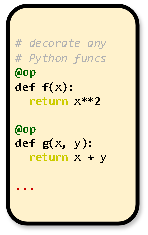
\includegraphics[width=\textwidth]{img/fig1.pdf}
% \caption{Add the \texttt{@op} decorator to any Python function to make it memoizable}
\end{subfigure}
\begin{subfigure}{0.35\textwidth}
\centering
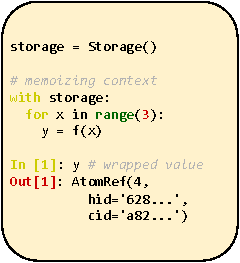
\includegraphics[width=\textwidth]{img/fig2.pdf}
% \caption{}
\end{subfigure}
\begin{subfigure}{0.4\textwidth}
\centering
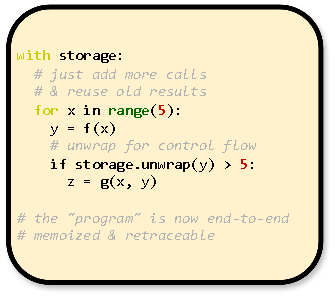
\includegraphics[width=\textwidth]{img/fig3.pdf}
% \caption{}
\end{subfigure}
\caption{Basic imperative usage of \texttt{mandala}. \textbf{Left}: add the \texttt{@op}
decorator to any Python functions to make them memoizable. \textbf{Middle}:
create a \texttt{Storage}, and use it as a context manager to automatically
memoize any calls to \texttt{@op}-decorated functions in the block. Memoized
functions return \texttt{Ref} objects, which wrap a value with two pieces of
metadata: a \emph{content ID}, which is a hash of the value of the
object, and a \emph{history ID}, which is a hash of the identity of the
\texttt{@op} that produced the \texttt{Ref} (if any), and the history IDs of the
\texttt{@op}'s inputs. \textbf{Right}: the storage context allows simple
incremental computation and recovery from failures. Here, we add more
computations while transparently reusing already computed values.}
\label{fig:basic-usage}
\end{figure}

In this paper we present \texttt{mandala}, our proposal for such a system. At
its core, it \textbf{integrates best data management practices} --- such as full
data provenance tracking, idempotent \& deterministic computation,
content-addressable versioning of code and its dependencies, and declarative
high-level data manipulation --- \textbf{into Python's already familiar syntax
and semantics} (Figures \ref{fig:basic-usage} and \ref{fig:cf}). The integration aims to be
maximally transparent and unobtrusive, so that the user can focus on the
\emph{essential complexity} (the scientific problem at hand), rather than on the
\emph{accidental complexity} (the data management tools used to solve it)
\citep{Brooks1987NoSB}.

The rest of this paper presents the design and main functionalities of
\texttt{mandala}, and is organized as follows: 
\begin{itemize}
\item In Section \ref{section:core-concepts}, we describe how memoization is
designed, how this allows memoized calls to be composed and memoized results to
be reused without storage duplication, and how this enables the \emph{retracing}
pattern of interacting with computational artifacts.
\item In Section \ref{section:cf}, we introduce the concept of a
\emph{computation frame}, which generalizes a dataframe by replacing columns
with a computational graph, and rows with individual computations that
(partially) follow this graph. Computation frames allow high-level exploration
and manipulation of the stored computation graph, such as adding the
creators/consumers of given values to the graph, deleting all computations that
depend on the calls captured in the frame, and restricting the frame to a
particular subgraph or subset of values with given properties.
\item In Section \ref{section:extra-features}, we describe some other features of
\texttt{mandala} necessary to make it a practical tool, such as optionally
storing elements of Python collections as separate values (enabling transparent
reuse of individual elements), caching of intermediate results, and a flexible
versioning system with dynamic dependency tracking.
\end{itemize}

Finally, we give an overview of related work in Section \ref{section:related-work}.

\section{Core Concepts}
\label{section:core-concepts}

\subsection{Memoization and the Computational Graph}

Memoization is a technique that stores the results of expensive function calls
to avoid redundant computation. \texttt{mandala} uses \emph{automatic}
memoization \citep{norvig1991techniques} which is applied via the combination of
a decorator (\texttt{@op}) and a context manager which specifies the
\texttt{Storage} object to use (Figure \ref{fig:basic-usage}). The memoization
can optionally be made persistent to disk, which is what you would typically want in a
long-running project. Any Python function can be memoized (as long as its inputs
and outputs are serializable by the \texttt{joblib} library); there is no
restriction on the type, number or naming scheme (positional, keyword, variadic)
of the arguments or return values.

\paragraph{\texttt{Call} and \texttt{Ref} objects, and content/history IDs.}
\texttt{Ref}s and \texttt{Call}s are the two main data structures in
\texttt{mandala}'s model of computations. When a call to an
\texttt{@op}-decorated function \texttt{f} is executed inside a storage context,
this results in the creation of 
\begin{itemize}
\item a \texttt{Ref} object for each input to the call. These wrap the `raw'
values passed as inputs together with content IDs (hashes of the Python objects)
and history IDs (hashes of the memoized calls that produced these values, if
any). If an input to the call is already a \texttt{Ref} object, it is passed
through as is; if it is a raw value, a new \texttt{Ref} object is created with a
`empty' history ID that is simply a hash of the content ID itself.
\item a \texttt{Call} object, which has pointers to the input and output
\texttt{Ref}s of the call to \texttt{f}, as well as a content ID for the call (a
hash of the identity of \texttt{f} and the content IDs of the input
\texttt{Ref}s) and a history ID (by analogy, a hash of the identity of
\texttt{f} and the history IDs of the inputs).
\item a \texttt{Ref} object for each output of the call. These are again
assigned content IDs by value, and history IDs by hashing the tuple (history ID
of the call, corresponding output name\footnote{Since Python functions don't
have designated output names, we instead generate output names automatically using the order in the tuple of return values.}).
\end{itemize}

\begin{wrapfigure}[23]{r}{0.5\textwidth}
    \centering
    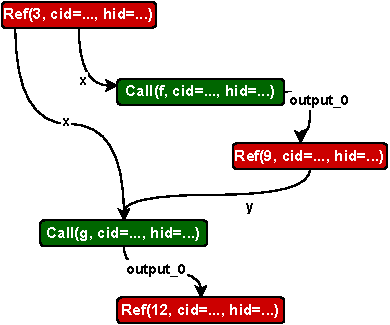
\includegraphics[width=\linewidth]{img/comp-graph.pdf}
    \caption{A part of the computaitonal graph built up by the calls in Figure
    \ref{fig:basic-usage}. The nodes are \texttt{Call} and \texttt{Ref} objects,
    and the edges are the inputs/output names connecting them.}
    \label{fig:comp-graph}
\end{wrapfigure}


The \texttt{Ref}s and the \texttt{Call} are then stored in the storage backend,
and the next time \texttt{f} is called on inputs that have the same
\emph{content} IDs, the stored \texttt{Call} is looked up to find the output
\texttt{Ref}s, which are then returned (possibly with properly updated history
IDs, if the call exists in storage by content ID only). The combination of all
stored \texttt{Call}s and \texttt{Ref}s across memoized functions form the
\textbf{computational graph} represented by the storage (Figure \ref{fig:comp-graph}). Importantly, the
`interesting' structure of this graph is built up automatically by the way the
user composes memoized calls.


The simultaneous use of content and history IDs has a few subtle advantages.
First, it allows for the \emph{de-duplication} of storage, as the same content
ID can be used to store the same value produced by different computations. For
instance, there may be many computaitions all producing the value $42$ (or a
large all-zero array), but only one copy of $42$ is stored in the backend. At
the same time, the history IDs allow us to distinguish between computations that
produced the same value, but in different ways. This avoids `parasitic' results
in declarative queries. For example, a call to \texttt{f} may result in 42, and
we may be interested in all computations that were called on this particular 42
returned by \texttt{f} and not on any other 42. Without history IDs, it would be
impossible to make this distinction in the stored computational graph.


\paragraph{Why memoization?} Memoization is an unusual choice for data
management systems, most of which are based on \emph{logging}, i.e. explicitly
pointing to the value to be saved and the address where it should be saved
(whether this is some kind of name or a file path). Basing data management on
memoization means that the `address' of a value is now implicit in the code that
produced it, and the value itself is stored in a shared storage backend. This has several advantages:
\begin{itemize}
\item it \textbf{eliminates the need to manually name artifacts}. This
eliminates a major source of accidental complexity: names are arbitrary,
ambiguous, and can drift away from the actual content of the value they point to
over time. On the other hand, names are not strictly necessary, because the
composition of memoized functions that produced a given value -- which must be specified anyway -- is already a canonical reference to it. 
\item it \textbf{organizes storage activities around a familiar and useful
interface -- the function call}. This automatically enforces the good practice
of partitioning code into functions, and eliminates extra `accidental' code to
save and load values explicitly. Furthermore, it synchronizes failures between
computation and storage, as the memoized calls are the natural points to
recover from.
\end{itemize}

The trade-off is that referring to values without reference to code that
produced or used them becomes difficult, because from the point of view of
storage the `identity' of a value is its place in the computational graph. We
discuss practical ways to overcome this in Section \ref{section:cf}.

\subsection{Retracing as a Versatile Imperative Interface to the Stored Computation Graph}
\label{subsection:retracing}

The compositional nature of memoization makes it possible to build complex
computations out of calls to memoized functions, turning the entire computation
into an end-to-end-memoized interface to its own intermediate results. The main
way to interact with such a computation is through \textbf{retracing}, which
means stepping through memoized code with the purpose of resuming from a
failure, loading intermediate values, or continuing from a particular point with
new computations. A small example of retracing is shown in Figure
\ref{fig:basic-usage} (right). 

This pattern is simple yet powerful, as it allows the user to interact with the
stored computation graph in a way that is adapted to their use case, and to
explore the graph in a way that is natural and familiar to them. It also
simplifies the management of state in an interactive environment such as a
Jupyter notebook, because it makes it very cheap to re-run cells.


\section{Computation Frames}
\label{section:cf}

\begin{figure}[h]
\centering
\begin{subfigure}{0.47\textwidth}
\centering
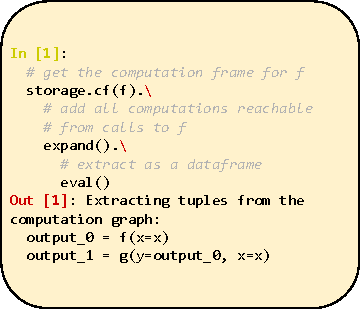
\includegraphics[width=\textwidth]{img/fig4.pdf}
\end{subfigure}
\begin{subfigure}{0.47\textwidth}
\centering
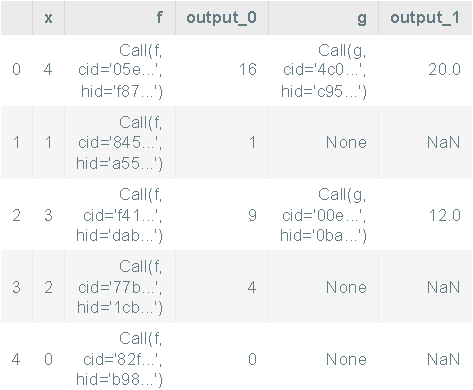
\includegraphics[width=\textwidth]{img/fig5.pdf}
\end{subfigure}
\caption{Basic declarative usage of \texttt{mandala} and an example of
computation frames. \textbf{Left}: continuing from Figure
\ref{fig:basic-usage}, we first create a computation frame from a single
function \texttt{f}, then expand it to include all calls that can be reached
from the memoized calls to \texttt{f} via their inputs/outputs, and finally
convert the computation frame into a dataframe. We see that this automatically
produces a computation graph corresponding to the computations found. \textbf{Right}:
the output of the call to \texttt{.eval()} from the left subfigure used to turn
the computaiton frame into a dataframe. The resulting table has columns for all
variables and functions appearing in the captured computation graph, and each
row correspond to a partial computation following this graph. The variable
columns contain values these variables take, whereas function columns contain
call objects representing the memoized calls to the respective functions. We see
that, because we call \texttt{g} conditional on the output of \texttt{f}, some
rows have nulls in the \texttt{g} column.}
\label{fig:cf}
\end{figure}

In order to be able to explore and manipulate the full stored computation graph,
patterns like retracing are insufficient, because they require the complete code
producing part of the graph to be available. Instead, we introduce the concept
of a \emph{computation frame}, which is a high-level declarative interface to
the stored computation graph. 

\subsection{Definition}
\label{subsection:cf-definition}
A computation frame (Figure \ref{fig:cf}) consists of the following data:
\begin{itemize}
\item \textbf{computation graph}: a directed graph $G=(V,F,E)$ where $V$ are
variables, $F$ are \texttt{@op}-decorated functions, and labeled edges $E$
connect from variables to functions using these variables as input (with the
edge label being the input name), and from functions to variables that are
outputs of these functions (with the edge label being the name of the output). An example is shown in Figure \ref{fig:comp-graph}.
\item \textbf{instance data}: for each variable $v\in V$, a set of history
IDs $H_v$ of \texttt{Ref}s corresponding to this variable, and for each function
$f\in F$ a set of history IDs $C_f$ of \texttt{Call}s to $f$ corresponding to
this node. 
\end{itemize}
Most importantly, this data is subject to the constraint that, if there exists a
call $c\in C_f$ where $f$ is connected via an input/output edge to some variable
$v$, then the value of $v$ corresponding to this call belongs to $H_v$. In other
words, when we look at all calls in $f\in F$, their inputs/outputs  must be
present in the variables connected to $f$ under the same input/output name. 

Intuitively, computation frames are `views' of the stored computation graph,
analogous to database views. In particular, they can be organized in a way that
is natural for a specific use case, may contain multiple references to the same
\texttt{Ref} or \texttt{Call} object, and do not necessarily contain all calls
to a given function. Formally speaking, there is a directed graph homomorphism
(a direction- and adjacency-preserving mapping from vertices to vertices and
edges to edges) from a computation frame's instance data to the full stored
computation graph.

\subsection{Basic Usage}
\label{subsection:cf-basic-usage}

The main advantage of computation frames is that they allow iterative
exploration of the computation graph, and high-level grouped operations over
computations with some shared structure. For example, we can use them for 
\begin{itemize}
\item \textbf{iteratively expanding the frame with functions that generated or
used existing variables}: this is useful for exploring the computation graph in
a particular direction, or for adding more context to a particular computation.
For example, in Figure \ref{fig:cf} (left), we start with a computation frame
containing only the calls to \texttt{f}, and then expand it to include all calls
that can be reached from the memoized calls to \texttt{f} via their
inputs/outputs, which adds the calls to \texttt{g} to the frame.
\item \textbf{converting the frame into a dataframe}: this is useful at the end
of an exploration, when we want to get a convenient tabular representation of
the captured computation graph. The table is obtained by collecting all terminal
\texttt{Ref}s in the frame's computational graph (i.e., those that are not
inputs to any function in the frame), computing their computational history in
the frame (grouped by variable), and joining the resulting tables over the
variables. This is shown in Figure \ref{fig:cf} (right). In particular, as shown
in the example, this step may produce nulls, as the computation frame can
contain computations that only partially follow the graph.
\item \textbf{performing high-level storage manipulations}: such as deleting all
calls captured in the frame as well as all calls that depend on them, available
using the \verb|.delete_calls()| method on the frame.
\end{itemize}

Computation frames are a powerful tool for exploring and manipulating the stored
computation graph, and we're excited to explore their full potential in future
work.

\section{Some Extra Features}
\label{section:extra-features}

\subsection{Data Structures}
\label{subsection:data-structures}

Python's native collections -- lists, dicts, sets -- can be memoized
transparently by \texttt{mandala}, using customized type annotations, e.g.
\texttt{MList[int]} inheriting from \texttt{List[int]}, \ldots. By applying this
type annotation, the collection is memoized so that its individual elements as
well as the collection itself are memoized as \texttt{Ref}s (with the collection
merely pointing to the \texttt{Ref}s of its elements to avoid duplication). 

\begin{wrapfigure}[18]{l}{0.45\textwidth}
    \centering
    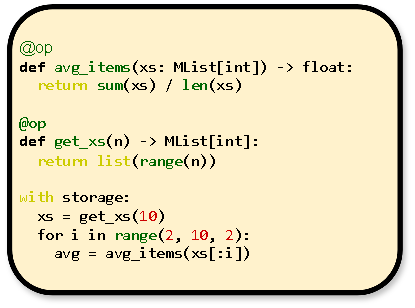
\includegraphics[width=\linewidth]{img/list.pdf}
    \caption{Illustration of native collection memoization in \texttt{mandala}.
    The custom type annotation \texttt{MList[int]} is used to memoize a list of
    integers as a list of pointers to element \texttt{Ref}s.}
    \label{fig:list}
\end{wrapfigure}

This is implemented fully on top of the core memoization machinery, using
`internal' \texttt{@op}s like e.g. \verb|__make_list__| which, given the
elements of a list as variadic inputs, generates a \texttt{ListRef} (subclass of
\texttt{Ref}) that points to the \texttt{Ref}s of the elements. In this way,
collections are naturally incorporated in the computation graph. These internal
\texttt{@op}s are applied automatically when a collection is passed as an
argument to a memoized function, or when a collection is returned from a
memoized function. The upshot is that collection elements can be reused
transparently, as shown in Figure \ref{fig:list}.

\subsection{Caching}
To speed up retracing and memoization, it is necessary to avoid frequent reads
and writes to the database backend. To this end, \texttt{mandala} implements a
fairly standard caching system that accumulates results in memory, with the
option to explicitly flush values to disk at once when the user decides, or
automatically at the end of a \texttt{mandala} context. Similarly, to speed up
retracing of existing calls, call metadata can be pre-loaded.

\subsection{Versioning}
\label{subsection:versioning}

It is crucial to have a flexible and powerful code versioning system in a data
management tool, as it allows the user to keep track of the evolution of their
computations, and to easily recover from mistakes. \texttt{mandala} provides the
option to use a versioning system with two main features:
\begin{itemize}
\item \textbf{content-addressed versioning} \citep{git}, where the version of a
function is a hash of its source code and the hashes of the functions it calls.
\item \textbf{dynamic dependency tracking}, where each function call traces the
functions it calls. This avoids the need for static analysis of the code to find
dependencies, which can result in many false positives and negatives, especially
in a dynamic language like Python.
\end{itemize}

A full discussion of the versioning system is beyond the scope of this paper,
but we refer the reader to a blog post by the author
\citep{makelov2023practical} for details and motivation.

\section{Related Work}
\label{section:related-work}

\texttt{mandala} combines ideas from several existing projects, but is unique in
the Pythonic way it makes complex memoized computations easy to query,
manipulate and version.

\paragraph{Memoization.} The \texttt{incpy} project \citep{guo2011using} enables
automatic persistent memoization of Python functions directly on the interpreter
level. The \texttt{funsies} project \citep{lavigne2021funsies} is a
memoization-based distributed workflow executor that uses a similar hashing
approach to \texttt{mandala} to keep track of which computations have already
been done. It works on the level of scripts (not functions), and lacks
queriability and versioning. \texttt{koji} \citep{maymounkov2018koji} is a
design for an incremental computation data processing framework that unifies
over different resource types (files or services). It also uses an analogous
notion of hashing to keep track of computations.

\paragraph{Computation Frames.} Computation frames are very closely related to
functors $\mathcal{F}:\mathscr{C}\to \underline{\mathbf{Set}}$ where
$\mathscr{C}$ is a finite category, and this perspective has been explored in
e.g. \citep{patterson2022categorical}.

\paragraph{Versioning.} The revision history of each function in the codebase is
organized in a `mini-git repository' that shares only the most basic features
with \texttt{git} \citep{git}: it is a content-addressable tree, where each edge
tracks a diff from the content at one endpoint to that at the other. Additional
metadata indicates equivalence classes of semantically equivalent contents.
Semantic versioning \citep{semver} is another popular code versioning system.
mandala is similar to semver in that it allows you to make backward-compatible
changes to the interface and logic of dependencies. It is different in that
versions are still labeled by content, instead of by `non-canonical' numbers.
The unison programming language \citep{lozano2017unison} represents functions by
the hash of their content (syntax tree, to be exact).

\section{Conclusion}
\label{section:conclusion}

\texttt{mandala} is being actively developed, and has the potential to
considerably simplify the way scientific data is managed and interacted with in
Python. The author has already used it extensively to manage several multi-month
machine learning projects, and has found it to be a very powerful tool for
managing complex computations. We hope that this paper has given a good overview
of the core concepts of \texttt{mandala}, and that the reader will be interested
in exploring the library further.


% bibliography
\bibliography{scipy}
\bibliographystyle{arxiv_template}

\end{document}